The \emph{\index{z-transform}{z-transform}} is a general frequency
domain representation of discrete-time signals. A special case of the
$z$-transform is the discrete-time Fourier transform.

The main benefit of the $z$-transform is that it allows us to use
algebraic manipulations of complex valued polynomials to study the
frequency domain behavior of discrete-time signals. This can simplify
calculations and provide further mathematical intuition. The
$z$-transform also provides a framework that can be used to derive
numerically efficient low-order filters\footnote{filters that require only a small 
number of computations to apply on signals}. The $z$-transform
also has applications, e.g., in statistics and statistical signal
processing.

\subsection{System function $\Hez$}

\tikzstyle{int}=[draw, minimum size=2em]
\tikzstyle{init} = [pin edge={to-,thin,black}]
\begin{marginfigure}
\begin{center}
  \begin{tikzpicture}[node distance=3cm,auto,>=latex']
    \node [int] (a) {LTI $h[n]$};
    \node (b) [left of=a, coordinate] {a};
%    \node (c) [below=a,node distance=3cm] {a};

%\node [int, pin={[init]above:$p_0$}] (c) [right of=a] {$\frac{1}{s}$};
    \node [coordinate] (end) [right of=a]{};
    \path[->] (b) edge node {$x[n]=z^n$} (a);
    %\path[->] (a) edge node {$v$} (c);
    \draw[->] (a) edge node {$\mathcal{H}(z)z^n$} (end) ;
\end{tikzpicture}
\end{center}
\caption{The motivation for the $z$-transform is studying how an LTI system modifies a signal $z^n$ with $z\in \mathbb{C}$.}
\end{marginfigure}

The \emph{\index{system function}{system function}} $\Hez$ provides an
alternative frequency domain representation of the frequency response
of LTI systems. We'll start by defining what this is.

Recall that a discrete-time LTI system can be represented as a
convolution of an input signal $x[n]$ with the impulse response $h[n]$
of the LTI system:
\begin{align}
y[n] &= \mathcal{T}\{x[n]\}\\
    &= h[n]*x[n]\\
     &= \sum_{k=-\infty}^{\infty} h[k] x[n-k]
\end{align}
The system function arises from investigating what is the output of
this LTI system when using an input signal of the form $x[n]=z^n$,
where $z\in \mathbb{C}$ is an arbitrary complex number. What happens
to this signal when it is fed into an LTI system? Let's find out:
\begin{align}
y[n] &= \mathcal{T}\{x[n]\}\\
     &= \sum_{k=-\infty}^{\infty} h[k] x[n-k]\\
     &= \sum_{k=-\infty}^{\infty} h[k] z^{n-k}\\
     &= \underbrace{\left(\sum_{k=-\infty}^{\infty} h[k] z^{-k}\right)}_{\Hez} z^n \\
     &= \Hez z^n.
\end{align}
The output signal is the original input signal $z^n$ multiplied with $\mathcal{H}(z)$. This term is called the \emph{\index{system
function}{system function}} of the LTI system:
\begin{equation}
\boxed{
\Hez = \sum_{k=-\infty}^{\infty} h[k] z^{-k}
}
\label{eq:system_function_eq}
\end{equation}
Sometimes the term \emph{\index{transfer function}{transfer function}}
is used instead of the system function\sidenote{The term transfer function is used e.g., by the SciPy $z$-transform functions.}. 
They both refer to $\mathcal{H}(z)$. 

The system function also happens to be a transformation called
the \emph{\index{$z$-transform}{$z$-transform}} of the signal $h[n]$. Recall
that this is similar to the frequency response of an LTI system, which
we investigated earlier. There we investigated the response of a
signal of the form $x[n]=A e^{i\hat{\omega}n}$ for a discrete-time LTI
system.

\if 0
If we set $z = e^{i\hat{\omega}}$ and substitute this with $z$ in
Equation \ref{eq:system_function_eq}, we get:
\begin{equation}
\He = \sum_{k=-\infty}^{\infty} h[k] e^{-i\hat{\omega}k}
\end{equation}
This is the frequency response $\He$ of an LTI system, or in other
words, the discrete-time Fourier transform of the impulse response
signal $h[n]$. Therefore, a special case of the $z$-transform is the
discrete-time Fourier transform.

\fi

\section{What is the meaning of $z^{n}$?}

\begin{marginfigure}
\begin{center}
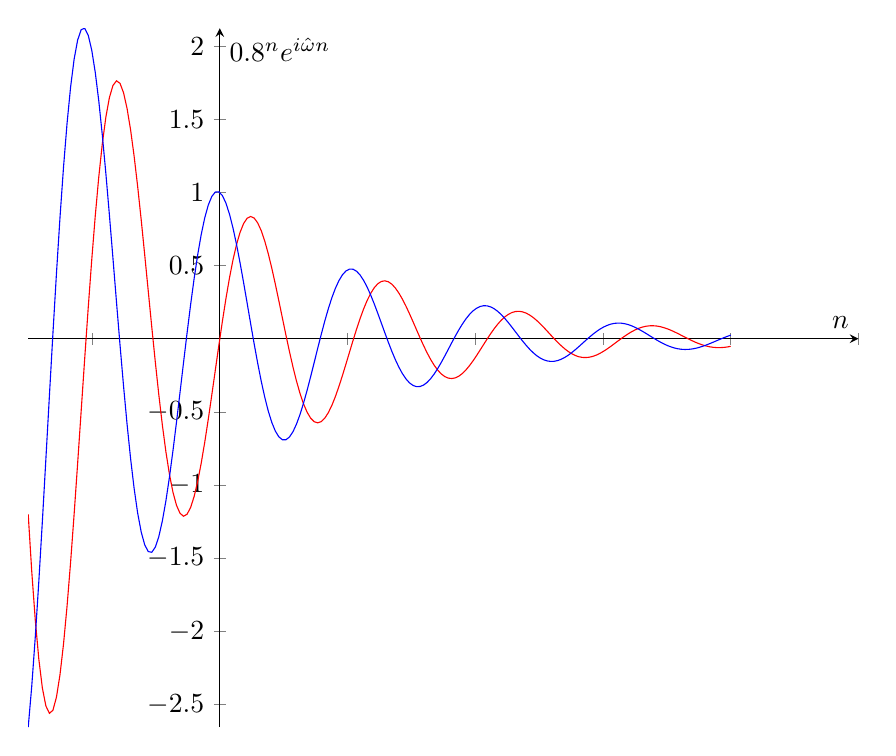
\begin{tikzpicture}
  \begin{axis}[ width=\textwidth,domain=(-3):(8),samples=200,
      xmin=-3,xmax=10, legend
      style={draw=none,at={(.99,.1)},anchor=south east}, xlabel={$n$},
      ylabel={$0.8^n e^{i\hat{\omega}n}$}, axis x line=middle, axis y
      line=middle, xticklabels=none] \addplot[red]
      {(0.7^x)*sin(deg(x*3))}; \addplot[blue]
      {(0.7^x)*cos(deg(x*3))}; \end{axis}
\end{tikzpicture}

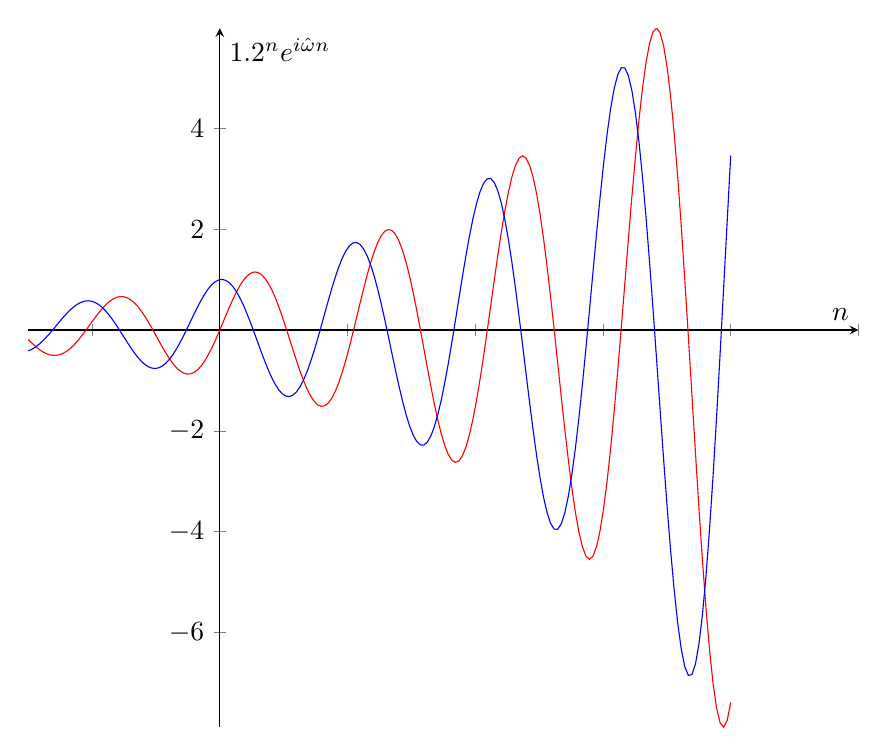
\begin{tikzpicture}
  \begin{axis}[width=\textwidth,domain=(-3):(8),samples=200, xmin=-3,xmax=10, 
      legend style={draw=none,at={(.99,.1)},anchor=south east},
      xlabel={$n$},
      ylabel={$1.2^n e^{i\hat{\omega}n}$},
      axis x line=middle, 
      axis y line=middle, 
      %    xtick={-2,0,10.0},
      xticklabels=none%{$-\pi$,0,$\pi$}    
    ]
    \addplot[red] {(1.3^x)*sin(deg(x*3))};
    \addplot[blue] {(1.3^x)*cos(deg(x*3))};
    \end{axis}
\end{tikzpicture}
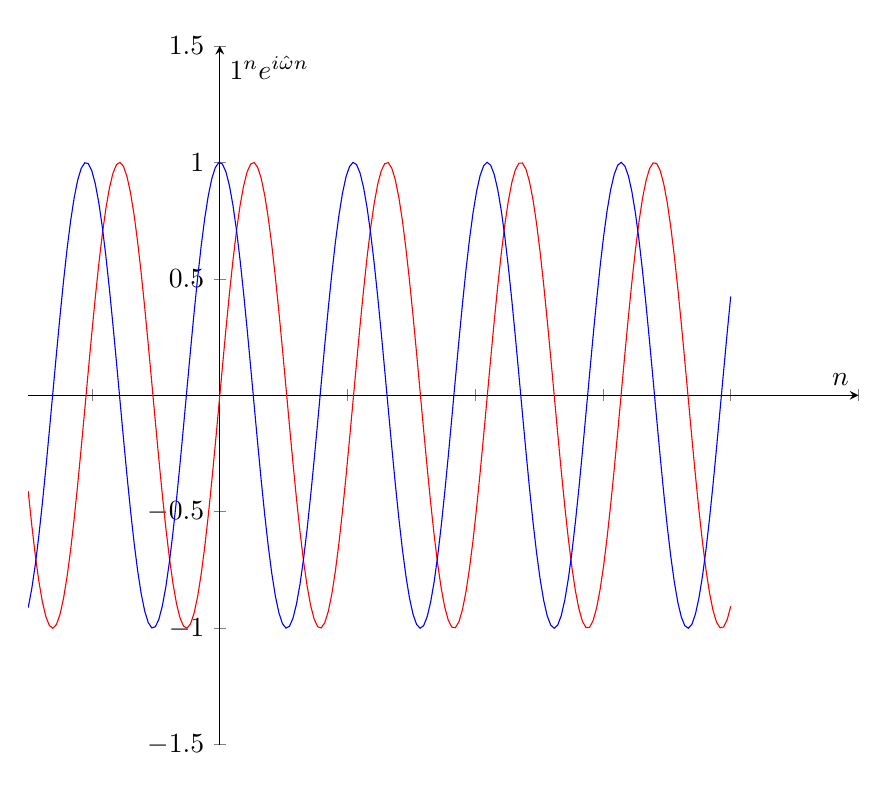
\begin{tikzpicture}
	\begin{axis}[width=\textwidth,domain=(-3):(8),samples=200, xmin=-3,xmax=10, ymax=1.5, ymin=-1.5,
            legend style={draw=none,at={(.99,.1)},anchor=south east},
            xlabel={$n$},
	    ylabel={$1^n e^{i\hat{\omega}n}$},
            axis x line=middle, 
            axis y line=middle, 
            %    xtick={-2,0,10.0},
            xticklabels=none%{$-\pi$,0,$\pi$}    
    ]
    \addplot[red] {(1.0^x)*sin(deg(x*3))};
    \addplot[blue] {(1.0^x)*cos(deg(x*3))};
    \end{axis}
\end{tikzpicture}
\end{center}
\caption{Several examples of the signal $z^{n}=A^n e^{i \hat{\omega} n}$ with different values of $A$.}
\label{fig:exp_sin_ex}
\end{marginfigure}

What does a signal of the form $x[n]=z^n$ look like? The variable
$z\in \mathbb{C}$ is a complex number. We can express a complex number
in polar form $z=A e^{i\hat{\omega}}$, where $A=|z|$ and
$\hat{\omega} = \angle z$. This means that:
\begin{equation}
\boxed{
z^{n}=A^n e^{i \hat{\omega} n}
}
\end{equation}
This signal is \index{exponentially decaying}{exponentially decaying}
when $A<1$, \index{exponentially growing}{exponentially growing} when
$A>1$, or constant in amplitude when $A=1$. The meaning of
$\hat{\omega}$ is the familiar normalized angular frequency in units
of radians per sample.

Figure \ref{fig:exp_sin_ex} shows several examples of a signal of the
form $z^{n}=A^n e^{i \hat{\omega} n} u[n]$. The unit step function
$u[n]$ is used to restrict the values of $z^n$ to be non-zero
only for positive values of $n$.

The signal $z^{n}$ is more general than just a complex sinusoidal
signal $e^{i \hat{\omega} n}$. It allows the amplitude of the signal to
exponentially grow, decay, or stay constant.
 

\section{Z-transform}
\usetikzlibrary{arrows,positioning} 
\tikzset{
    %Define standard arrow tip
    >=stealth',
    %Define style for boxes
    punkt/.style={
           rectangle,
           rounded corners,
           draw=black, very thick,
           text width=6.5em,
           minimum height=2em,
           text centered},
    % Define arrow style
    pil/.style={
           ->,
           thick,
           shorten <=2pt,
           shorten >=2pt,}
}

\subsection*{Forward transform}
The \index{forward $z$-transform}{forward $z$-transform} $X(z)$ of an arbitrary discrete-time signal $x[n]$ is
defined as:
\begin{equation}
\boxed{
X(z) = \mathcal{Z}\{x[n]\} = \sum_{k=-\infty}^{\infty} x[k] z^{-k}.}
\label{zf}
\end{equation}
The $z$-transform is not necessarily defined everywhere, as the sum
may not converge for some values of $z$. The set of points
$S_{\mathrm{ROC}}$ on the complex plane where the sum $X(z)$ converges
to a finite value is known as the \emph{\index{region of
    convergence}{region of convergence}}:
\begin{equation}
S_{\mathrm{ROC}} = \left\{z \in \mathbb{C} :  |X(z)| < \infty\right\}
\end{equation}
In terms of filter design, the region of convergence indicates the set
of signals for which a filter provides a finite output. 

\begin{marginfigure}
\begin{center}
\begin{tikzpicture}
	\begin{axis}[width=\textwidth, 
	             domain=(0):(2*3.145),
	             samples=100,
	             xmin=-1.6,
	             axis equal,
	             xmax=1.6, 
	             ymin=-1.6,
	             ymax=1.6,
	             legend style={draw=none,at={(.99,.1)},anchor=south east},
                     xlabel={$\mathrm{Re}\{z\}$},
	             ylabel={$\mathrm{Im}\{z\}$},
                     axis x line=middle, 
                     axis y line=middle
%                     yticklabels=none,
 %                    xticklabels=none
          ]
    \addplot[domain=0:7,samples=100,color=blue]({sin(deg(x))},{cos(deg(x))});
    \node at (axis cs:1.3,1.0) {$z=e^{i\hat{\omega}}$};          
    \end{axis}
    \end{tikzpicture}
\end{center}
\caption{The function $z=e^{i\hat{\omega}}$ is a parametric curve for a circle on the complex plane.}
\end{marginfigure}

\subsection{Reverse transform}
The \index{inverse $z$-transform}{inverse $z$-transform} is defined as
a \index{contour integral}{contour integral}:
\begin{equation}
\boxed{
x[n] = \mathcal{Z}^{-1}\{X(z)\} =  \frac{1}{2 \pi i} \oint_{C} X(z) z^{n-1} dz}.
\label{izteq}
\end{equation}
Here $C$ is a closed loop that encircles the origin within the region
of convergence.

Solving the inverse $z$-transform directly using this formula requires
the use of contour integration\sidenote{This topic is beyond the scope
of this course. You will not need to know how to solve
Equation \ref{izteq} in the exam.}. However, one typically does not
need to use this formula, because with practical signal processing
applications, it is nearly always possible to algebraically manipulate
the $z$-transform polynomial $X(z)$ in such a way that it is possible to
use a table of elementary $z$-transform pairs to obtain an inverse
$z$-transform symbolically.

\subsection{Relationship to the discrete-time Fourier transform}

It is possible to determine the DTFT of a signal using a $z$-transform
of the signal $X(z)$. This is done by substituting
$z=e^{i\hat{\omega}}$. In other words, evaluating the $z$-transform
along the unit circle.

\begin{marginfigure}
\begin{center}
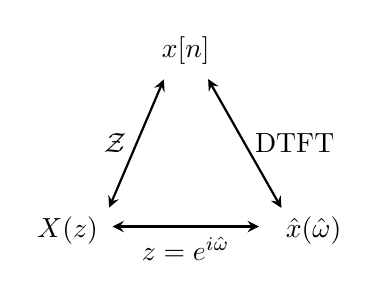
\begin{tikzpicture}[
      scale=0.5,
      level/.style={thick},
      virtual/.style={draw opacity=0},
      trans/.style={thick,<->,shorten >=2pt,shorten <=2pt,>=stealth},
      oneway/.style={thick,->,shorten >=2pt,shorten <=2pt,>=stealth},
      classical/.style={thin,double,<->,shorten >=4pt,shorten <=4pt,>=stealth}
    ]
    % Draw the energy levels.
  %  \draw[level] (2cm,-2em) -- (0cm,-2em) node[left] {a};
  %  \draw[level] (2cm,11em) -- (4cm,11em) node[midway,above] {b};
%    \draw[level] (4cm,-11em) -- (6cm,-11em) node[right] {$x[n]$};
    % Draw the virtual levels.
    \draw[virtual] (2cm,8em) -- (4cm,8em) node[midway,above] {$x[n]$};
    
    \draw[virtual] (5.5cm,-5em) -- (7cm,-5em) node[midway,above] {$\hat{x}(\hat{\omega})$};
    
    \draw[virtual] (1cm,-5em) -- (-1cm,-5em) node[midway,above] {$X(z)$};
    % Draw the transitions.
    \draw[trans] (1cm,-2em) -- (2.5cm,8em) node[midway,left] {$\mathcal{Z}$};
    
    \draw[trans] (3.5cm,8em) -- (5.5cm,-2em) node[midway,right] {DTFT};
    \draw[trans] (1cm,-3em) -- (5cm,-3em) node[midway,below] {$z=e^{i\hat{\omega}}$};
    \end{tikzpicture}
\end{center}
\caption{The $z$-transform $X(z)$ evaluated on the unit circle $z=e^{i\hat{\omega}}$ corresponds to the discrete-time Fourier transform. }
\end{marginfigure}

Recall the definition of the $z$-transform:
\begin{equation}
X(z) = \sum_{k=-\infty}^{\infty} x[k] z^{-k}.
\label{zfr}
\end{equation}
If we replace $z=e^{i\hat{\omega}}$, we obtain the discrete-time Fourier transform:
\begin{equation}
\hat{x}(\hat{\omega}) = \sum_{k=-\infty}^{\infty} x[k] e^{-i\hat{\omega}k}.
\label{zfr2}
\end{equation}
In a sense, the $z$-transform is a more general frequency domain
representation of a discrete-time signal than a discrete-time Fourier
transform, as a subset of the $z$-transform is the discrete-time Fourier
transform.

One application is that the $z$-transform of the impulse response $h[n]$ of
an LTI system can be used to obtain the frequency response of an LTI
system:
\begin{equation}
  \boxed{
    \mathcal{H}(\hat{\omega}) = \mathcal{H}(z)|_{z=e^{i\hat{\omega}}}
    }
  \end{equation}
In other words, if one knows the system function, it is possible to evaluate the frequency response.

\subsection{Linearity}
The $z$-transform is a linear transformation:
\begin{equation}
\boxed{
\alpha_1 x_1[n] + \alpha_2 x_2[n] \xleftrightarrow{\mathcal{Z}} \alpha_1 X_1(z) + \alpha_2 X_2(z)}.
\end{equation}
To show this, let's investigate the following linear combination of
signals $x[n]=\alpha_1 x_1[n] + \alpha_2 x_2[n]$. The $z$-transform for
$x[n]$ is:
\begin{align}
X(z) & = \sum_{n}(\alpha_1 x_1[n] + \alpha_2 x_2[n])z^{-n} \\
     & = \alpha_1 \sum_n x_1[n]z^{-n} + \alpha_2 \sum_n x_2[n] z^{-n} \\
     & = \alpha_1 X_1(z) + \alpha_2 X_2(z). \qed
\end{align}
The result is a linear combination of the $z$-transforms of the two
individual signals that form the signal $x[n]$.


\section{Time-shifted unit impulse $\delta[n-n_0]$}

\begin{marginfigure}
\begin{center}
\begin{tikzpicture}
	\begin{axis}[width=7cm,
	             domain=(-3):(8),
	             samples=12,
	             xmin=-3,
	             xmax=12, 
	             ymin=-0.2,
	             ymax=1.5,
	             legend style={draw=none,at={(.99,.1)},anchor=south east},
        xlabel={$n$},
	    ylabel={$\delta[n-n_0]$},
        axis x line=middle, 
    axis y line=middle, 
    xtick={0,4},
    xticklabels={$0$,$n_0$}    
    ]
    \addplot+[ycomb]{(x==4)};
%    \node at (axis cs:9,0.5) [center,fontsize={\Large}]{$\hdots$};          
    \end{axis}
    \end{tikzpicture}
\end{center}
\caption{A time-shifted unit impulse is a basic building block of
  arbitrary signals. If you know the $z$-transform of this signal, you
  can determine the $z$-transform of an arbitrary finite-length
  discrete-time signal, as it will be a linear combination of time-shifted unit impulses.}
\end{marginfigure}

One of the elementary $z$-transform pairs is a time-shifted unit impulse:
\begin{equation}
  \boxed{
    x[n]=\delta[n-n_0] \xleftrightarrow{\mathcal{Z}} X(z) = z^{-n_0}.
      \label{eq:z_shifted_unit_impulse}
  }
\end{equation}
A \index{time-shifted unit impulse}{time-shifted unit impulse} is a
basic building block of discrete-time signals, which have a finite
number of non-zero elements.

This can be easily obtained using Equation \ref{zf} for the forward $z$-transform:
\begin{align}
X(z) &= \mathcal{Z}\{\delta[n-n_0]\} \\
     &= \sum_{k=-\infty}^{\infty} \delta[k-n_0] z^{-k}\\
     &= z^{-n_0}\qed
\end{align}
The special case of this is the unit impulse $\delta[n]$, which
results in $\mathcal{Z}\{\delta[n]\}=1$.


It is also possible to evaluate the reverse transform of:
\begin{equation}
  X(z)=z^{-n_0},
\end{equation}
by using Equation \ref{izteq}. We select the unit circle $|z|=1$ as
the contour of integration $C$. It is easy to see that the unit circle
is in the region of convergence, as the system function is of constant
magnitude along the unit circle $|e^{-i\hat{\omega}n_0}|=1$.

\begin{marginfigure}
\begin{center}
\begin{tikzpicture}
	\begin{axis}[width=\textwidth, 
	             domain=(0):(2*3.145),
	             samples=100,
	             xmin=-1.6,
	             axis equal,
	             xmax=1.6, 
	             ymin=-1.6,
	             ymax=1.6,
	             legend style={draw=none,at={(.99,.1)},anchor=south east},
                     xlabel={$\mathrm{Re}\{z\}$},
	             ylabel={$\mathrm{Im}\{z\}$},
                     axis x line=middle, 
                     axis y line=middle
%                     yticklabels=none,
 %                    xticklabels=none
          ]
    \addplot[domain=0:7,samples=100,color=blue]({sin(deg(x))},{cos(deg(x))});
    \node at (axis cs:1.3,1.0) {$z=e^{i\hat{\omega}}$};          
    \end{axis}
    \end{tikzpicture}
\end{center}
\caption{The function $z=e^{i\hat{\omega}}$ is a parametric curve for a circle on the complex plane.}
\end{marginfigure}

Integration along the unit circle is achieved with variable
substitution $z=e^{i\hat{\omega}}$. By sweeping the parameter
$\hat{\omega}$ between 0 and $2\pi$, the variable $z$ draws a unit
circle on the complex plane. This is the closed curve $C$.

With the chosen variable substitution, we find that $dz/d\hat{\omega}
= i e^{i\hat{\omega}}$ and we can substitute the infinitesimal $dz$ with
$i e^{i\hat{\omega}} d\hat{\omega}$.

The limits of integration, which result in a closed counterclockwise
loop around the contour of integration, are: $[0,2\pi]$. We now have
everything that we need to inverse $z$-transform $X(z)=z^{-n_0}$:
\begin{align}
x[n] &= \mathcal{Z}^{-1}\{ z^{-n_0} \} \\
     &= \frac{1}{2\pi i}\oint_C z^{-n_0} z^{n-1} dz \\
     &= \frac{1}{2\pi i}\oint_C z^{n-n_0-1}  dz 
     \end{align}
Let's now insert $dz=ie^{i\hat{\omega}}d\hat{\omega}$, $z=e^{i\hat{\omega}}$ and use the limits $0,2\pi$ for $\hat{\omega}$:
     \begin{align}
x[n] &= \frac{1}{2\pi i} \int_0^{2\pi} e^{i\hat{\omega} (n-n_0-1)} i e^{i\hat{\omega}} d\hat{\omega} \\
&= \frac{1}{2\pi } \int_0^{2\pi} e^{i\hat{\omega} (n-n_0)}   d\hat{\omega}.
\end{align}
Let's investigate two cases. In the first case $n \ne n_0$. It is easy to see that this integral is zero when $n \ne n_0$. This is
because $n-n_0$ is an integer. The second case is when $n=n_0$, we then get:
\begin{align}
x[n_0] &= \frac{1}{2\pi}\int_{0}^{2\pi} d\hat{\omega} \\
 &= 1.
\end{align}
Combining these two results, we get:
\begin{equation}
    x[n] = \delta[n-n_0]\qed
\end{equation}
%This forms the elementary \index{z-transform of a time-shifted unit impulse}{z-transform of a time-shifted unit impulse}
%\begin{align}
%\boxed{
%  x[n]=\delta[n-n_0] \xleftrightarrow{\mathcal{Z}} X(z)=z^{-n_0}.
%  
%}
%\end{align}
%This is one of the most commonly encountered z-transform pairs.

\section{Arbitrary signals of finite length}

By using Equation \ref{eq:z_shifted_unit_impulse} and linearity, you
can forward and reverse $z$-transform an arbitrary signal $x[n]$ with a
finite number of non-zero values:
\begin{equation}
  \boxed{
    x[n] = \sum_{k=0}^{N}  b_k \delta[n-n_k] \xleftrightarrow{\mathcal{Z}} X(z) = \sum_{k=0}^{N}  b_k z^{-n_k}
    \label{eq:fir_z_transform}
    }
\end{equation}
Here $n_k$ denotes the time-shift of the $k$th non-zero element
$x[n_k]=b_k$. A large fraction of practical signals are of this form, so this is a very useful formula.

\subsection{Example: System function of an FIR filter}

\begin{marginfigure}
\begin{center}
\begin{tikzpicture}
	\begin{axis}[width=7cm,
	             domain=(-3):(9),
	             samples=13,
	             xmin=-3,
	             xmax=12, 
	             ymin=-3.0,
	             ymax=4.0,
	             legend style={draw=none,at={(.99,.1)},anchor=south east},
            xlabel={$n$},
	    ylabel={$h[n]$},
        axis x line=middle, 
    axis y line=middle, 
    xtick={3,5,7},
    xticklabels={$3$,$5$,$7$}    
    ]
    \addplot+[ycomb]{(x==3)-2*(x==5)+3*(x==7)};
    \end{axis}
    \end{tikzpicture}
\end{center}
\caption{A finite impulse response $h[n]$.}
\label{fig:fir_ex_h_1}
\end{marginfigure}

A discrete-time LTI system $y[n]=\mathcal{T}\{x[n]\}$ is defined using the following \emph{\index{difference equation}{difference equation}}:
\begin{equation}
y[n] = x[n-3] - 2 x[n-5] + 3 x[n-7].
\end{equation}
This is a finite impulse response filter (shown in Figure \ref{fig:fir_ex_h_1}), with the following impulse response:
\begin{equation}
h[n]=\delta[n-3]-2\delta[n-5]+3\delta[n-7].
\end{equation}
Using Equation \ref{eq:fir_z_transform} we get the following system function ($z$-transform of the LTI system impulse response):
\begin{align}
\Hez &= z^{-3} - 2 z^{-5} + 3 z^{-7}.
\end{align}
We can also multiply this with $z^{7}/z^{7}$ and obtain a polynomial
fraction with more familiar positive valued exponents of the following
form:    
\begin{align}
\Hez &= \frac{z^{4} - 2 z^{2} + 3}{z^{7}}
\end{align}
This means that the system function in this case is a polynomial
fraction, with a fourth order polynomial on the numerator and a seventh order polynomial on the denominator.

\if 0
The numerator of the system function is a second order polynomial. The \emph{fundamental theorem of algebra} states that a polynomial of degree $N$ has $N$ zeros. In the case of our example, the system function has 2 zeros, which can be in this case found using the quadratic formula:
\begin{equation}
\Hez = \frac{1}{z^2}\left(z^2 -3z + 2 \right) = \frac{1}{z^2}\left(z-1\right)\left(z-2\right)
\end{equation}
The zeros of the system function are: $z_1=1$ and $z_2=2$. We will later see how analysis of the system function polynomial can be used to analyze the properties of this system. 

Recall that the second order polynomial solution formula is for a polynomial zeros $a z^2 + bz + c=0$ is:
\begin{equation}
z = \frac{-b \pm \sqrt{b^2-4ac}}{2a}.
\end{equation}

\fi
\subsection{Example: Algebraic inverse z-transform}

Given a system function $\Hez$, it is possible to go back into time
domain and to determine the impulse response $h[n]$ of an FIR filter
using \index{simple algebraic manipulations}{simple algebraic
manipulations}, instead of the more involved contour integration
discussed earlier. From the impulse response, it is then possible to
reconstruct a difference equation describing the output of the
discrete-time LTI system as a function of the input signal.

For example, let's say that we have a system function of the following form:
\begin{equation}
  \mathcal{H}(z) = \frac{3z^{3} - 2 z + 1}{z^{2}}
  \label{eq:poly_ex}
\end{equation}


\noindent We can find the inverse $z$-transform of $\Hez$ purely by algebraic
manipulation. First, let's write Equation \ref{eq:poly_ex} as:
\begin{equation}
  \mathcal{H}(z) = 3z^{1} - 2z^{-1}  + z^{-2}.
\end{equation}
We can now use Equation \ref{eq:fir_z_transform}, to obtain the impulse
response, which is the inverse $z$-transform of $\Hez$:
\begin{equation}
h[n] = 3\delta[n+1] - 2\delta[n-1] + \delta[n-2].
\end{equation}
This is shown in Figure \ref{fig:algebraic_ex1}. We can see that the
difference equation for this LTI system can be written as
\begin{equation}
y[n] = 3x[n+1]-2x[n-1]+ x[n-2].
\end{equation}
\begin{marginfigure}
\begin{center}
\begin{tikzpicture}
	\begin{axis}[width=7cm,
	             domain=(-3):(9),
	             samples=13,
	             xmin=-3,
	             xmax=12, 
	             ymin=-3.0,
	             ymax=4.0,
	             legend style={draw=none,at={(.99,.1)},anchor=south east},
            xlabel={$n$},
	    ylabel={$h[n]$},
        axis x line=middle, 
    axis y line=middle, 
    xtick={3,5,7},
    xticklabels={$3$,$5$,$7$}    
    ]
    \addplot+[ycomb]{3*(x==-1)-2*(x==1)+(x==2)};
    \end{axis}
    \end{tikzpicture}
\end{center}
\caption{A finite impulse response $h[n]$.}
\label{fig:algebraic_ex1}
\end{marginfigure}


\section{Time-shift theorem}
The \index{time-shift theorem}{time-shift theorem} allows us to obtain
the $z$-transform of a time delayed signal using polynomial multiplication:
\begin{equation}
  \boxed{
    y[n] = x[n-n_0] \xleftrightarrow{\mathcal{Z}} Y(z) = z^{-n_0}X(z)
    }
\end{equation}
Here $X(z)$ is the $z$-transform of signal $x[n]$, and $Y(z)$ is the
$z$-transform of signal $x[n-n_0]$. We'll use this property later to
prove the convolution theorem for the $z$-transform.

It is easy to see that the time-shift property follows from the
definition of the $z$-transform. Let us assume that the $z$-transform of
the signal $x[n]$ is $X(z)$:
\begin{equation}
X(z) = \sum_{k=-\infty}^{\infty} x[k] z^{-k}.
\end{equation}
If we now delay $x[k]$ by $n_0$ samples, and look at the $z$-transform
of the delayed signal $y[n]=x[n-n_0]$, we get:
\begin{align}
Y(z) &= \sum_{k=-\infty}^{\infty} y[k] z^{-k}\\
    &= \sum_{k=-\infty}^{\infty} x[k-n_0] z^{-k}\\
%     &= \sum_{\ell=-\infty}^{\infty} x[\ell] z^{-\ell}z^{-n_0}\\
     &= z^{-n_0}\sum_{\ell=-\infty}^{\infty} x[\ell] z^{-\ell}\\
     &= z^{-n_0}X(z)\qed
\end{align}
We used variable substitution: $k-n_0 = \ell$. 



\section{Convolution theorem}
The \index{convolution theorem}{convolution theorem} is of fundamental
importance for theoretical and practical applications in signal
processing. This theorem states that \emph{convolution in time domain 
is multiplication in frequency domain}. We've already encountered
this with Fourier transforms. Now we'll introduce the $z$-transform
equivalent.

\tikzstyle{int}=[draw, minimum size=2em] \tikzstyle{init} = [pin
  edge={to-,thin,black}]
\begin{marginfigure}
\begin{center}
  \begin{tikzpicture}[node distance=3cm,auto,>=latex']
    \node [int] (a) {LTI};
    \node (b) [left of=a, coordinate] {a};
%    \node (c) [below=a,node distance=3cm] {a};

%\node [int, pin={[init]above:$p_0$}] (c) [right of=a] {$\frac{1}{s}$};
    \node [coordinate] (end) [right of=a]{};
    \path[->] (b) edge node [above]{$x[n]$} (a);
    \path[->] (b) edge node [below]{$X(z)$} (a);

%\path[->] (a) edge node {$v$} (c);
    \draw[->] (a) edge node [below]{$Y(z)=\Hez X(z)$} (end) ;
    \draw[->] (a) edge node [above]{$y[n]=h[n]*x[n]$} (end) ;

\end{tikzpicture}
\end{center}
\caption{One consequence of the convolution theorem is that the $z$-transform of the output of an LTI system $Y(z)$ is the $z$-transform of the input signal $X(z)$ multiplied with the system function $\Hez$.}
\end{marginfigure}

If the signal $a[n]$ is a convolution of signals $b[n]$ and $c[n]$ and the
$z$-transforms of these signals are $A(z)$, $B(z)$, and $C(z)$, we
have the following $z$-transform rule:
\begin{equation}
  \boxed{
    a[n]=b[n]*c[n] \xleftrightarrow{\mathcal{Z}} A(z) = B(z) C(z).
  }
\end{equation}
One application of this is that we can use the $z$-transform to investigate the $z$-domain representation of the output of an LTI system:
\begin{equation}
  \boxed{
    y[n]=h[n]*x[n] \xleftrightarrow{\mathcal{Z}} Y(z) = \Hez X(z)
    }
\end{equation}
Here $\Hez$ is the system function, which is the $z$-transform of the impulse response $h[n]$.

\begin{proof}
The proof of the $z$-transform convolution theorem is as follows. We start with the definition of a convolution operation:
\begin{equation}
a[n] = b[n]*c[n] = \sum_{k} b[k] c[n-k].
\end{equation}
$z$-transforming $a[n]$, one obtains:
\begin{marginfigure}
\begin{center}
\begin{tikzpicture}
	\begin{axis}[width=6cm, 
	             domain=(-3):(8),
	             samples=12,
	             xmin=-3,
	             xmax=4, 
	             ymin=-1.2,
	             ymax=1.5,
	             legend style={draw=none,at={(.99,.1)},anchor=south east},
        xlabel={$n$},
	    ylabel={$h[n]$},
        axis x line=middle, 
    axis y line=middle, 
    xtick={0,4},
    xticklabels=none%{$0$,$n_0$}    
    ]
    \addplot+[ycomb] coordinates {
    (-2,0)             
    (-1,0)
    (0,1)
    (1,-1)
    (2,0)
    (3,0)
    };
%    \node at (axis cs:9,0.5) [center,fontsize={\Large}]{$\hdots$};          
    \end{axis}
    \end{tikzpicture}
    \begin{tikzpicture}
	\begin{axis}[width=6cm, 
	             domain=(-3):(8),
	             samples=12,
	             xmin=-3,
	             xmax=5, 
	             ymin=-0.2,
	             ymax=4.0,
	             legend style={draw=none,at={(.99,.1)},anchor=south east},
        xlabel={$n$},
	    ylabel={$x[n]$},
        axis x line=middle, 
    axis y line=middle, 
    xtick={0,4},
    xticklabels=none%{$0$,$n_0$}    
    ]
        \addplot+[ycomb] coordinates {
    (-2,0)             
    (-1,0)
    (0,2)
    (1,1)
    (2,3)
    (3,0)
    (4,0)
    };
    
%    \addplot+[ycomb]{(x==4)};
%    \node at (axis cs:9,0.5) [center,fontsize={\Large}]{$\hdots$};          
    \end{axis}
    \end{tikzpicture}
\end{center}
\begin{center}
    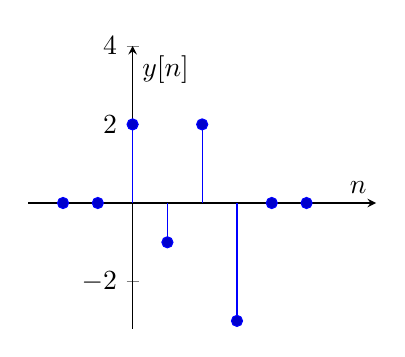
\begin{tikzpicture}
	\begin{axis}[width=6cm, 
	             domain=(-3):(8),
	             samples=12,
	             xmin=-3,
	             xmax=7, 
	             ymin=-3.2,
	             ymax=4.0,
	             legend style={draw=none,at={(.99,.1)},anchor=south east},
        xlabel={$n$},
	    ylabel={$y[n]$},
        axis x line=middle, 
    axis y line=middle, 
    xtick={0,4},
    xticklabels=none%{$0$,$n_0$}    
    ]
        \addplot+[ycomb] coordinates {
    (-2,0)             
    (-1,0)
    (0,2)
    (1,-1)
    (2,2)
    (3,-3)
    (4,0)
    (5,0)
    };
    
%    \addplot+[ycomb]{(x==4)};
%    \node at (axis cs:9,0.5) [center,fontsize={\Large}]{$\hdots$};          
    \end{axis}
    \end{tikzpicture}
\end{center}
\caption{A convolution of signals $h[n]$ (top) and $x[n]$ (middle) is $y[n]=x[n]*h[n]$ (bottom).}
\label{fig:two_signals_zt_conv}
\end{marginfigure}
\begin{align}
A(z) &= \sum_{n} (b[n]*c[n]) z^{-n} \\
     &= \sum_{n} \left(\sum_{k} b[k] c[n-k]\right) z^{-n}.
     \\
     &=  \sum_{k} b[k] \underbrace{\left(\sum_{n} c[n-k] z^{-n}\right)}_{z^{-k}C(z)}\\
     &= \sum_{k}b[k] z^{-k} C(z)\\
&= \underbrace{\left(\sum_{k}b[k] z^{-k}\right) }_{B(z)} C(z)\\
     &= B(z) C(z)
\end{align}
\end{proof}
We rely on the time-shift theorem to obtain the $z$-transform of the
delayed signal $b[n-k]$.

\subsection{Example: convolution in $z$-domain}

Let $h[n] = \delta[n] - \delta[n-1]$ and $x[n]=2\delta[n]+\delta[n-1]+3\delta[n-2]$. These signals are shown in Figure \ref{fig:two_signals_zt_conv}.

In this case, $\Hez = 1 - z^{-1}$ and $X(z)=2+z^{-1}+3z^{-2}$. What is
$y[n]=h[n]*x[n]$? We can of course directly solve this in time domain,
but we can often more efficiently solve this in frequency domain.

We can obtain the result of the convolution using polynomial calculations and $z$-transforms. The $z$-transform of $y[n]$ is:
\begin{align}
Y(z) & = \Hez X(z) \\
     & = (1-z^{-1})(2+z^{-1}+3z^{-2})\\
     &= 2 - z^{-1} + 2z^{-2} - 3 z^{-3}\\
     &=y[0]z^0 +y[1] z^{-1} + y[2]z^{-2} +y[3]z^{-3}.
\end{align}
Since $Y(z)=\sum_n y[n] z^{-n}$, it follows that:
\begin{equation}
y[n]=2\delta[n]-\delta[n-1]+2\delta[n-2]-3\delta[n-3].
\end{equation}
The signal $y[n]$ is shown on the bottom panel of Figure \ref{fig:two_signals_zt_conv}.

\subsection{Example: Two filter cascade}

When two LTI systems are cascaded as shown in Figure
\ref{fig:cascade1}, the system is mathematically described by
\begin{equation}
w[n] = \sum_{\ell} h_1[\ell]x[n-\ell] = h_1[n]*x[n]
\end{equation}

\begin{marginfigure}
\begin{center}
  \begin{tikzpicture}[node distance=2cm,auto,>=latex']
    \node [int] (a) {$h_1[n]$};
    \node [int] (two) [right of=a] {$h_2[n]$};
    \path[->] (a) edge node [above] {$w[n]$} (two);
%     \node (b) [left of=two, coordinate] {a};
%    \node (c) [below=a,node distance=3cm] {a};

%\node [int, pin={[init]above:$p_0$}] (c) [right of=a] {$\frac{1}{s}$};
    \node [coordinate] (end) [right of=two]{};
\node [coordinate] (start) [left of=a]{};
\path[->] (start) edge node [above]{$x[n]$} (a);
\path[->] (two) edge node [above]{$y[n]$} (end);

%\path[->] (end) edge node [above]{$x[n]$} (a);

%\path[->] (b) edge node {$x[n]=z^n$} (a);
    %\path[->] (a) edge node {$v$} (c);
    %\draw[->] (a) edge node {$y[n]$} (end) ;
\end{tikzpicture}
\end{center}
\caption{A system that consists of two LTI systems connected in series (cascade).}
\label{fig:cascade1}
\end{marginfigure}

\begin{marginfigure}
\begin{center}
  \begin{tikzpicture}[node distance=3cm,auto,>=latex']
    \node [int] (a) {$h_1[n]*h_2[n]$};
    \node [coordinate] (end) [right of=a]{};
\node [coordinate] (start) [left of=a]{};
\path[->] (start) edge node [above]{$x[n]$} (a);
\path[->] (a) edge node [above]{$y[n]$} (end);

%\path[->] (end) edge node [above]{$x[n]$} (a);

%\path[->] (b) edge node {$x[n]=z^n$} (a);
    %\path[->] (a) edge node {$v$} (c);
    %\draw[->] (a) edge node {$y[n]$} (end) ;
\end{tikzpicture}
\end{center}
\end{marginfigure}
\noindent and
\begin{align}
  y[n] &= \sum_k h_2[k]w[n-k] \\
  &= h_2[n]*w[n] \\
  &= h_2[n]*(h_1[n]*x[n]).
\end{align}
Because convolution is associative, $a*(b*c) =(a*b)*c$, the two
convolutions can be combined as follows:
\begin{align}
y[n] &= h_2[n]*(h_1[n]*x[n])\\
 &= \underbrace{(h_1[n]*h_2[n])}_{h[n]} *x[n].
\end{align}
Which is equivalent to a single convolution by a combined LTI system
with an impulse response that is a convolution of two impulse
responses $h[n]=h_1[n]*h_2[n]$. In $z$-domain, the equivalent system
function that combines the two systems is:
\begin{equation}
h[n] = h_1[n] * h_2[n] \xleftrightarrow{\mathcal{Z}} \Hez = \mathcal{H}_1(z) \mathcal{H}_2(z).
\end{equation}
and the $z$-transform of the output $y[n]$ is:
\begin{equation}
Y(z) = \mathcal{H}_1(z)\mathcal{H}_2(z) X(z) = \Hez X(z).
\end{equation}

\section{FIR filters as cascaded first order systems}
It is possible to view an arbitrary finite impulse response filter as
a \index{cascade of first order filters}{cascade of first order
  filters}.

Let's assume that all the non-zero elements of the impulse response
of a FIR filter lie in the range $n \in \{0,\hdots,N\}$. If this is not the
case, we can always shift the impulse response in time so that the
first non-zero element of the impulse response is at sample index
$n=0$ (time-shift theorem).

The impulse response is then: 
\begin{equation}
  h[n] = \sum_{k=0}^{N} b_k \delta[n-k].
\end{equation}
And the $z$-transform is the following polynomial fraction:
\begin{align}
  \Hez &=  b_0 + b_1 z^{-1} + b_2 z^{-2} + \cdots b_N z^{-N} \\
       &=  z^{-N} (b_0z^{N} + b_1 z^{N-1} + b_2 z^{N-2} + \cdots b_N) 
\end{align}
The \emph{\index{fundamental theorem of algebra}{fundamental theorem
    of algebra}} states that a polynomial of degree $N$ has $N$
roots when counting with multiplicity. This means that we can represent the polynomial on the right-hand side of
$\mathcal{H}(z)$ in the following form:
\begin{align}
    \Hez  &= z^{-N} \prod_{k=1}^{N} (z-\alpha_k)\\
          &=  \prod_{k=1}^{N} (1-\alpha_k z^{-1})\\
          &= \prod_{k=1}^{N}\mathcal{H}_k(z).
\end{align}
In the second line, we have distributed $z^{-N}$ into the
product. Here $\alpha_k$ is a root of the $N$th order polynomial
$\mathcal{H}(\alpha_k)=0$.

We can see that the FIR filter is a product of elementary polynomials:
\begin{equation}
  \mathcal{H}_k(z) = 1-\alpha_k z^{-1}.
 \end{equation}
The convolution theorem says that convolution in time domain is
equivalent to multiplication in frequency domain. This means that
$\Hez$ is the result of a convolution of $N$ first order system
functions $\mathcal{H}_k(z)=1-\alpha_k z^{-1}$.

We can use the inverse $z$-transform on these systems to obtain the impulse
response of each first order filter:
\begin{equation}
  h_k[n] = \mathcal{Z}^{-1}\{\mathcal{H}_k(z)\} = \delta[n]-\alpha_k \delta[n-1]
\end{equation}
The full impulse response $h[n]$ is the result of these first order filters convolved together:
\begin{equation}
h[n] = h_1[n]*h_2[n]*h_3[n]*\cdots*h_{N}[n].
\end{equation}
This means that an FIR filter of arbitrary length can be decomposed
into elementary first order FIR filters. It is often easy to
analytically study how the individual first order filters behave (e.g.,
which signals each filter attenuates).


\section{Zeros of the system function of an FIR filter}
The system function of an FIR filter $\Hez$ is a polynomial. The
\emph{zeros} of the system function $\Hez$ are values $z=\alpha_k$, where
the system function evaluates to zero: $\mathcal{H}(\alpha_k) = 0$.

The location of the zeros determine the frequency domain behavior of
an FIR system. This allows us to use analysis of complex valued polynomials
to investigate the frequency domain behavior of LTI systems.

A zero of the system function means that the LTI system will
completely eliminate a signal of the form $x[n]=\alpha_k^{n}$, i.e.,
the amplitude of the output of the LTI system will be
$|\mathcal{T}\{\alpha_k^{n}\}|=0$.

\subsection{Example: First order FIR filter}

Consider the first order LTI system:
\begin{equation}
  y[n] = x[n] - x[n-1]
\end{equation}
This has an impulse response:
\begin{equation}
  h[n] = \delta[n] - \delta[n-1].
\end{equation}
And the system function is a first order polynomial:
\begin{equation}
  \mathcal{H}(z) = 1-z^{-1}.
\end{equation}
This is a first order polynomial with one zero at $z^{-1}=1$. In other
words, $\alpha_1=1$.

This means that if we feed in a constant (DC) signal $x[n]=\alpha_1^{n}=1$, the
system will completely filter out this signal. This makes sense, as
this system is a simple high-pass filter, which we have already
studied before in the discrete-time Fourier transform chapter. 

\section{Example: Third order FIR filter}

\begin{marginfigure}
\begin{center}
\begin{tikzpicture}
	\begin{axis}[width=7cm,
	             domain=(-3):(9),
	             samples=13,
	             xmin=-3,
	             xmax=12, 
	             ymin=-3.0,
	             ymax=4.0,
	             legend style={draw=none,at={(.99,.1)},anchor=south east},
            xlabel={$n$},
	    ylabel={$h[n]$},
        axis x line=middle, 
    axis y line=middle, 
    xtick={0,1,2,3},
    xticklabels={$0$,$1$,$2$,$3$}    
    ]
    \addplot+[ycomb]{(x==0)-2*(x==1)+2*(x==2)-(x==3)};
    \end{axis}
    \end{tikzpicture}
\end{center}
\caption{A finite impulse response $h[n]$ of a third order system.}
\end{marginfigure}

Let's look at a more complicated system. Consider the following system:
\begin{equation}
y[n]= x[n]-2x[n-1]+2x[n-2]-x[n-3].
\end{equation}
This is an FIR filter with the following impulse response:
\begin{equation}
h[n]= \delta[n]-2\delta[n-1]+2\delta[n-2]-\delta[n-3].
\end{equation}
This has a $z$-transform of the form 
\begin{equation}
\Hez = 1-2z^{-1} + 2z^{-2} - z^{-3}.
\end{equation}
This is a third order polynomial. Based on the fundamental theorem of algebra, this polynomial has three zeros. These zeros are at $\alpha_1=1$,
$\alpha_2=e^{i\frac{\pi}{3}}$, and $\alpha_3=e^{-i\frac{\pi}{3}}$. You can find
this using one of the many solution strategies for finding the roots
of a polynomial\sidenote[][-1cm]{It may be helpful to convert
  the polynomial into a form with positive exponents: $\Hez =
  z^{-3}(z^3 -2z^{2} + 2z^1 - 1)$ and to solve for $z^3 -2z^{2} + 2z^1
  - 1=0$ using a symbolic calculator such as Wolfram alpha. You don't need to make it a priority to learn how to solve higher order polynomials using pencil and paper. We have computers for that.}. Figure \ref{fig:pole_zero_third_order} shows the
locations of these zeros, marked with blue circles, on the complex
plane.


With the help of the roots of the polynomial, we can now write the
polynomial in the following form:
\begin{align}
\Hez &= (1-z^{-1})(1-e^{i\frac{\pi}{3}}z^{-1})(1-e^{-i\frac{\pi}{3}}z^{-1}).
\end{align}
This can also be viewed as a cascade of three different first order FIR filters:
\begin{align}
  \Hez &= \mathcal{H}_1(z) \mathcal{H}_2(z) \mathcal{H}_3(z)\\
       &= (1-z^{-1})(1-e^{i\frac{\pi}{3}}z^{-1})(1-e^{-i\frac{\pi}{3}} z^{-1} )
\end{align}
Using the $z$-transform, we can find the impulse responses of the individual filters: $h_1[n]=\delta[n]-\delta[n-1]$, $h_2[n]=\delta[n]-e^{i\frac{\pi}{3}}\delta[n-1]$, $h_3[n]=\delta[n]-e^{-i\frac{\pi}{3}}\delta[n-1]$. 
The cascaded filter equivalent to $h[n]$ is shown below.

\begin{figure}
\begin{center}
  \begin{tikzpicture}[node distance=2cm,auto,>=latex']
%    \node [int] (one) {$h_1[n]$};
    \node [int] (two)  {$h[n]$};
 %   \node [int] (three) [right of=two] {$h_3[n]$};

\node [coordinate] (end) [right of=two]{};
\node [coordinate] (start) [left of=two]{};

%\path[->] (one) edge node {}  (two);
\path[->] (two) edge node {} (end);

\path[->] (start) edge node [above]{$x[n]$} (two);
\path[->] (two) edge node [above]{$y[n]$} (end);

  %  \path[->] (a) edge node [above] {$w[n]$} (two);
%     \node (b) [left of=two, coordinate] {a};
%    \node (c) [below=a,node distance=3cm] {a};

%\node [int, pin={[init]above:$p_0$}] (c) [right of=a] {$\frac{1}{s}$};

%\path[->] (end) edge node [above]{$x[n]$} (a);

%\path[->] (b) edge node {$x[n]=z^n$} (a);
    %\path[->] (a) edge node {$v$} (c);
    %\draw[->] (a) edge node {$y[n]$} (end) ;
  \end{tikzpicture}
\end{center}
\begin{center}
  \begin{tikzpicture}[node distance=2cm,auto,>=latex']
    \node [int] (one) {$h_1[n]$};
    \node [int] (two) [right of=one] {$h_2[n]$};
    \node [int] (three) [right of=two] {$h_3[n]$};

\node [coordinate] (end) [right of=three]{};
\node [coordinate] (start) [left of=one]{};

\path[->] (one) edge node {}  (two);
\path[->] (two) edge node {} (three);

\path[->] (start) edge node [above]{$x[n]$} (one);
\path[->] (three) edge node [above]{$y[n]$} (end);

  %  \path[->] (a) edge node [above] {$w[n]$} (two);
%     \node (b) [left of=two, coordinate] {a};
%    \node (c) [below=a,node distance=3cm] {a};

%\node [int, pin={[init]above:$p_0$}] (c) [right of=a] {$\frac{1}{s}$};

%\path[->] (end) edge node [above]{$x[n]$} (a);

%\path[->] (b) edge node {$x[n]=z^n$} (a);
    %\path[->] (a) edge node {$v$} (c);
    %\draw[->] (a) edge node {$y[n]$} (end) ;
\end{tikzpicture}
\end{center}
\end{figure}

\begin{marginfigure}[-5cm]
\begin{center}
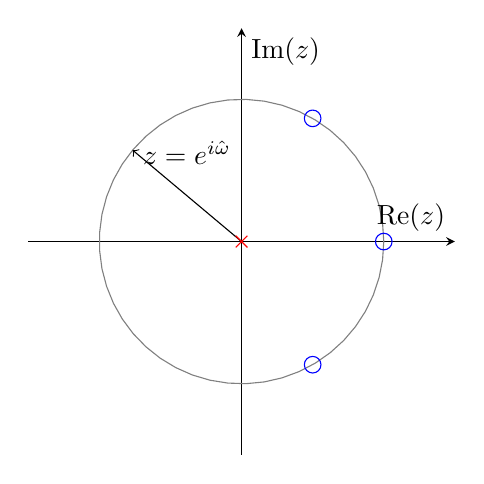
\begin{tikzpicture}
	\begin{axis}[axis equal, ymin=-1.5,xmin=-1.5,ymax=1.5,xmax=1.5,  ticks=none,
    xlabel=$\mathrm{Re}(z)$,
    ylabel=$\mathrm{Im}(z)$, axis lines = middle, width=7cm, height=7cm]
	\addplot [gray,domain=0:2*pi,samples=50]({cos(deg(x))},{sin(deg(x))});

\addplot [blue, mark = o,mark size=3pt] coordinates {( {cos(60)}, {sin(60)} )} {};   
\addplot [blue, mark = o,mark size=3pt] coordinates {( {cos(60)}, {sin(-60)} )} {};   

\addplot [blue, mark = o,mark size=3pt] coordinates {( {cos(0)}, {sin(0)} )} {};   

\addplot [red, mark = x,mark size=3pt] coordinates {( {0}, {0} )} {};   

\addplot [black,->] coordinates { (0,0) ( {cos(140)}, {sin(140)} ) };

\node at (axis cs:{0.5*cos(140)},{0.5*sin(140)+0.3}) {$z=e^{i\hat{\omega}}$};

%  \draw[draw=black] (axis cs:0.2,0) arc [radius=0.5cm,start angle=0,end angle=140]
 % node[midway,above right,inner sep=3pt,font={\footnotesize}]{$\hat{\omega}$};

% \node at (axis cs:0.9,1.4) {$z$};

% \node at (axis cs:0.9,-1.4) {$z^*$};

 %\node at (axis cs:0.25,0.7) [font={\footnotesize}]{$|z|$};

\end{axis}
\end{tikzpicture}
\end{center}
\caption{Locations of the three zeros
  ($\alpha_k=\{e^{i\frac{\pi}{3}n},e^{-i\frac{\pi}{3}n},1\}$) of
    $\mathcal{H}(z)$ in the complex plane are marked with blue
    circles. In this case, they all coincide with the unit circle.}
\label{fig:pole_zero_third_order}
\end{marginfigure}

The first filter $h_1[n]$ will completely remove a signal of the form
$x[n]=\alpha_1^n = 1$. The second will completely remove signals of the
form $x[n]=\alpha_2^n = e^{i\frac{\pi}{3}n}$, and the third filter will
remove signals of the form $x[n]=\alpha_3^n = e^{-i\frac{\pi}{3}n}$. This
filter completely removes three spectral components of the input
signal with normalized angular frequencies $\hat{\omega}_1=0$,
$\hat{\omega}_2=\frac{\pi}{3}$, and $\hat{\omega}_3=-\frac{\pi}{3}$.

\subsection{Plotting $\He$ on the complex plane}
In order to investigate what the system function $\mathcal{H}(z)$
looks like, I've written some Python code to plot the magnitude and
phase of the system function $\Hez$ on the complex plane for various
values of $z$. This code is shown in Listing
\ref{lst:third_order}. The plot is shown in Figure
\ref{fig:third_order_pz}.

\begin{marginfigure}
\begin{center}
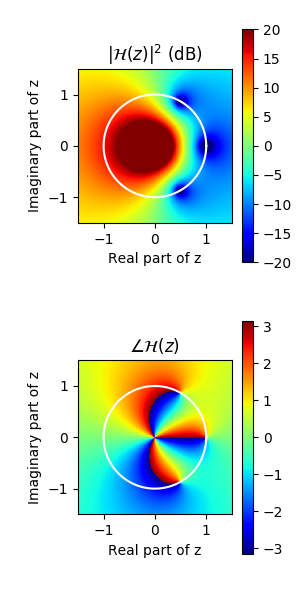
\includegraphics[width=\textwidth]{code/025_system_function/z_mag_angle.png}
\end{center}
\caption{The magnitude and phase angle of the system function plotted on the complex plane. The unit circle is shown in white.}
\label{fig:third_order_pz}
\end{marginfigure}

From this plot, one can see that $|\mathcal{H}(z)|$ obtains very low
values near the locations of the zeros of $\mathcal{H}(z)$. This means
that signals with normalized frequencies near $\hat{\omega}_1=0$,
$\hat{\omega}_2=\frac{\pi}{3}$, and $\hat{\omega}_3=-\frac{\pi}{3}$
are also reduced in amplitude as a result of the filtering operation.

The magnitude of $\Hez$ is larger than unity on the left-hand side of
the plot. This means that complex sinusoidal signals with sufficiently
high normalized angular frequencies are amplified by the system.


\lstinputlisting[language=Python,caption={\texttt{025\_system\_function/third\_order.py}},label=lst:third_order]{code/025_system_function/third_order.py}

\subsection{Frequency response $\He$}

In order to obtain the frequency response, evaluate $\Hez$ on the unit
circle $z=e^{i\hat{\omega}}$ for $\hat{\omega}\in[-\pi,\pi]$:
\begin{equation}
\He = (1-e^{-i\hat{\omega}})(1-e^{i(\frac{\pi}{3}-\hat{\omega})})(1-e^{-i(\frac{\pi}{3}+\hat{\omega})}) )
\end{equation}
The magnitude response $|\mathcal{H}(\hat{\omega})|$ is shown in Figure
\ref{fig:mag_resp_third}. This is a high-pass filter. Compare
$|\mathcal{H}(\hat{\omega})|$ with the values of $\Hez$ on the unit
circle, shown in on the top panel of Figure \ref{fig:third_order_pz}.


\begin{marginfigure}
\begin{center}
\begin{tikzpicture}
  \begin{axis}[ width=\textwidth,domain=(-3.14):(3.14),samples=200,
      xmin=-3.14,xmax=3.14, ymin=0.0,ymax=6.0, legend
      style={draw=none,at={(.99,.1)},anchor=south east},
      xlabel={$\hat{\omega}$},
      ylabel={$|\mathcal{H}(\hat{\omega})|$},
      axis x line=middle, axis y
      line=middle,
      xtick={-3.14,-1.047,0,1.047,3.14},
      xticklabels={$-\pi$,$-\frac{\pi}{3}$,$0$,$\frac{\pi}{3}$,$\pi$}
    ]
    \addplot[blue] {abs(2*2*2*sin(deg(x/2.0))*(sin(deg(0.5*(3.14/3.0-x))))*(sin(deg(0.5*(3.14/3.0+x)))))};
    
\end{axis}
\end{tikzpicture}
\end{center}
\caption{The magnitude response $|\mathcal{H}(\hat{\omega})|$ for the third order FIR filter.}
\label{fig:mag_resp_third}
\end{marginfigure}

The zeros of the system function, that lie on the unit circle $z=e^{i\hat{\omega}}$, correspond to the frequencies at which the gain of the system is zero. Thus, complex sinusoids at these frequencies are blocked. 


\section{Blocking filters}

The factorization of a filter can be used to design a \index{blocking
  filter}{filter} that blocks certain frequencies. A filter of the
form:
\begin{equation}
  \Hez = z^{-n_0}\prod_{k=1}^{N} (1-\alpha_k z^{-1})
  \label{eq:blocking_filter}
\end{equation}
blocks all signals of form $\alpha_k^n$. By selecting values of
$\alpha_k = e^{i\hat{\omega}_k}$, we can make a filter that blocks
complex sinusoidal signals $x[n]=e^{i\hat{\omega}_k n}$ with
frequencies $\hat{\omega}_k$, as we saw in the previous example. The
term $z^{-n_0}$ is an arbitrary time shift for this filter, which
doesn't affect the locations of the zeros of the system function.

\subsection{Example: blocking filter for a real-valued sinusoidal signal}

Let's design a filter that blocks a 50 Hz power line signal. We'll assume that this signal is sinusoidal:
\begin{equation}
  x[n]=\cos(\hat{\omega}_0 n) = \frac{1}{2}(e^{i\hat{\omega}_0 n}+e^{-i\hat{\omega}_0 n})
\end{equation}
If our sampling rate is $f_s=10^3$ Hz, a 50 Hz frequency would
correspond to a normalized angular frequency of $\hat{\omega}_0=2\pi
50/f_s = 0.1\pi$ radians per sample.

Because our signal has two spectral components, we need to filter out
normalized angular frequencies $\hat{\omega}=\pm 0.1\pi$. This would
correspond to zeros of the system function at $\alpha_1=e^{i0.1\pi}$
and $\alpha_2=e^{-i0.1\pi}$. We now have a filter description:
\begin{align}
\Hez & = (1-e^{-i 0.1 \pi} z^{-1})(1-e^{i 0.1 \pi} z^{-1}) \\
     &= 1 - (e^{-i0.1\pi} + e^{i0.1\pi})z^{-1} + (e^{-i0.1\pi} e^{i0.1\pi})z^{-2}\\
      &=1 - 2\cos(0.1\pi)z^{-1} + z^{-2}
\end{align}
This filter has an impulse response:
\begin{equation}
h[n] = \delta[n] -2\cos(0.1\pi)\delta[n-1] + \delta[n-2]
\end{equation}
and system function description:
\begin{equation}
y[n] = x[n] - 2\cos(0.1\pi)x[n-1]+x[n-2].
\end{equation}
This is a simple filter that will completely remove a pure 50 Hz
sinusoidal signal. You can expand on this to, e.g., build a filter that
blocks harmonics of 50 Hz.



\section{Running average filter}
\label{r_avg_z}

In the frequency response chapter, we analyzed the frequency response
of the \index{running average}{running average} filter. Now we will
analyze the $z$-transform of the same filter. 

This running average filter with $M=2N+1$ is defined using the
following system definition:
\begin{equation}
y[n] = \frac{1}{M}\sum_{k=-N}^{N} x[n-k].
\end{equation}
This system has the following impulse response:
\begin{equation}
h[n] = \frac{1}{M}\sum_{k=-N}^{N} \delta[n-k].
\end{equation}
The $z$-transform of this filter is:
\begin{align}
\Hez &= \sum_{k=-\infty}^{\infty} h[k]z^{-k}, \\
     &= \frac{1}{M}\sum_{k=-N}^{N} z^{-k}.
\end{align}
\begin{marginfigure}[15cm]
  \begin{center}
    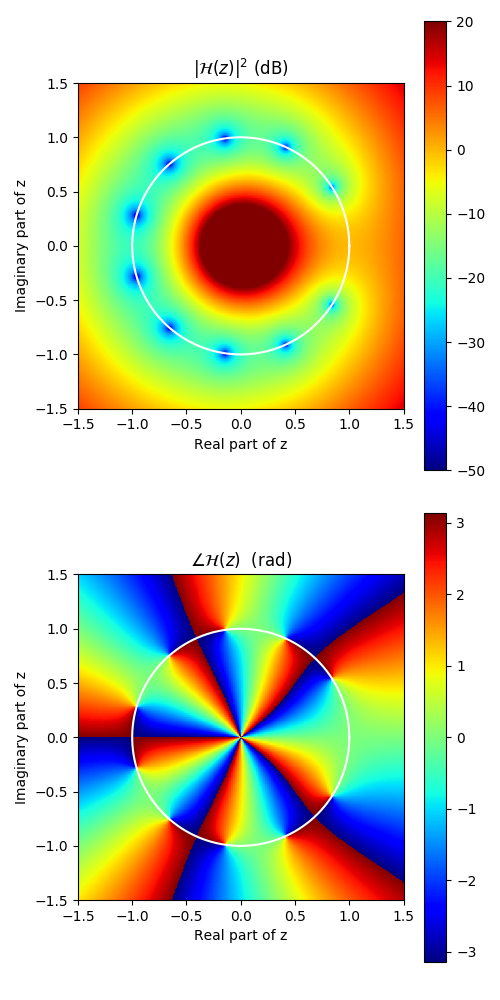
\includegraphics[width=\textwidth]{code/025_system_function/z_mag_angle_rm.png}
\end{center}
\caption{Above: The running average system function magnitude
  $|\mathcal{H}(z)|$ plotted on the complex plane. The $M-1$ zeros of
  the system function are evenly distributed
  $\alpha_k=e^{i\frac{2\pi}{M}k}$ with $k\in {1,2,\cdots,M-1}$. These
  are the frequencies that are perfectly removed by the filter. The unit
  circle $e^{i\hat{\omega}}$ is denoted with a white line. Below: The phase angle of the system function corresponding to a running average filter.}
\label{fig:rma_l20}
\end{marginfigure}
\noindent This is a \emph{\index{geometric series}{geometric series}}, which we can solve by our usual method. We obtain:
\begin{align}
\Hez &= \frac{1}{M}\frac{z^{N} - z^{-(N+1)}}{1-z^{-1}}.
\end{align}
Multiplying the right-hand side with $z^{N+1}/z^{N+1}$ gives:
\begin{align}
  \Hez &= \frac{1}{M}\frac{z^{2N+1} - 1}{z^{N}(z-1)}\\
       &= \frac{1}{M}\frac{z^{M} - 1}{z^{N}(z-1)}
\end{align}
The system function is zero when $z^{M} -1=0$, or $z^M = 1$. Since $1 =
e^{i2\pi k}$ for $k\in\mathbb{Z}$, it follows that the roots of the
$M$th order polynomial are $\alpha_k=e^{i\frac{2\pi}{M}k}$. This has
$M$ unique values when $k\in [0,1,2,\cdots, M-1]$.

We can now express the system function in factorized form:
\begin{align}
\Hez &= \frac{1}{M} \frac{1}{(z-1)z^{N}}\prod_{k=0}^{M-1}(z-e^{i\frac{2\pi}{M}k}) \\
 &= \frac{1}{M} \frac{1}{\cancel{(z-1)}z^{N}}\cancel{(z-1)}\prod_{k=1}^{M-1}(z-e^{i\frac{2\pi}{M}k}) \\
 &= \frac{1}{M} \frac{1}{z^{N}} \prod_{k=1}^{M-1}(z-e^{i\frac{2\pi}{M}k}) 
\end{align}
Notice that one of the zeros (for $k=0$) of the denominator polynomial coincides
with a zero of the numerator. This means that this root
of the system function polynomial cancels out.

Finally, we multiply with $z^{-(M-1)}/z^{-(M-1)}$ to obtain:
\begin{align}
\Hez &= \frac{1}{M} z^{N} \prod_{k=1}^{M-1}(1-e^{i\frac{2\pi}{M}k}z^{-1}).
\end{align}
We can see that this the same form as Equation
\ref{eq:blocking_filter}. This means that the running average filter
is actually a set of blocking filters which blocks complex sinusoidal
signals $x[n]=e^{i\frac{2\pi}{M}kn}$ with normalized angular frequencies
$\hat{\omega}_k=\frac{2\pi}{M}k$ with $k=[1,2,\cdots,M-1]$. The term
$z^{N}$ means that there is a time-shift (negative delay) by $N$ samples.

The magnitude of the running average system function $|\Hez|$ is shown
in Figure \ref{fig:rma_l20} for $N=5$ ($M=2N+1 = 11$). This system
function has 10 nulls at complex valued positions
$\alpha_k=e^{i\frac{2\pi}{11}k}$ with $k\in {1,2,\cdots,10}$. They are
all along the unit circle (shown with a white circle). Only the region
near $z=1$ doesn't have a null. This corresponds to the pass-band
region of this filter. Figure \ref{fig:rma_l20} also shows the phase
angle of the same system function.
\begin{marginfigure}[5cm]
\begin{center}
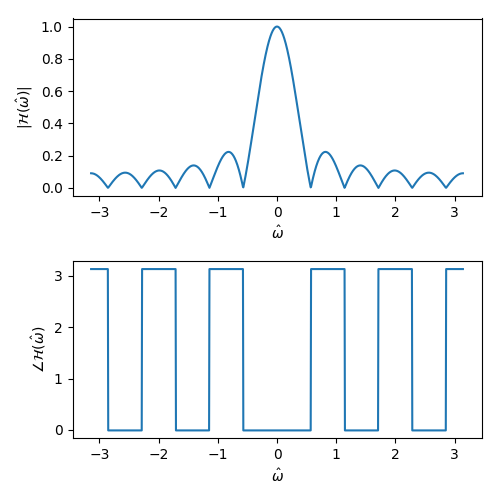
\includegraphics[width=\textwidth]{code/025_system_function/rma_magresp.png}
\end{center}
\caption{The magnitude and phase response of the running average
  filter. Within the main lobe of the low-pass filter pass band, the
  filter introduces no phase shift. The phase then alternates between
  0 and $\pi$ within the sidelobes.}
\label{fig:magresp}
\end{marginfigure}

If we evaluate the value of the system function on the unit circle
$z=e^{i\hat{\omega}}$, we obtain the magnitude and phase response of
the system. The magnitude and phase response shown in Figure
\ref{fig:magresp} looks exactly like the one we obtained earlier using
a discrete-time Fourier transform for the same running average filter.



\if 0
\section{Running average filter}
\label{r_avg_z}

In the frequency response chapter, we analyzed the frequency response
of the \index{running average}{running average} filter. Now we will
analyze the z-transform of the same filter. In this case, we'll use a
causal filter, which averages $L$ values of the input signal.

This running average filter is defined using the following definition:
\begin{equation}
y[n] = \frac{1}{L}\sum_{k=0}^{L-1} x[n-k]
\end{equation}
This system has the following impulse response:
\begin{equation}
h[n] = \frac{1}{L}\sum_{k=0}^{L-1} \delta[n-k].
\end{equation}
The z-transform of this filter is:
\begin{align}
\Hez &= \sum_{k=-\infty}^{\infty} h[k]z^{-k} \\
     &= \frac{1}{L}\sum_{k=0}^{L-1} z^{-k} 
\end{align}
This is a \emph{\index{geometric series}{geometric series}}. We can solve it using the following manipulations:
\begin{align}
\Hez &= \frac{1}{L}\sum_{k=0}^{L-1} z^{-k} ~~~~~~| \cdot z^{-1}\\
z^{-1}\Hez &= \frac{1}{L}\sum_{k=1}^{L} z^{-k}
\end{align}
If we now subtract the first line from the second line, we obtain:
\begin{align}
\Hez - z^{-1}\Hez &= \frac{1}{L}(1 - z^{-L})\\
\Hez(1 - z^{-1}) &= \frac{1}{L}(1 - z^{-L})\\
\Hez &= \frac{1}{L}\frac{1 - z^{-L}}{1-z^{-1}}.
\end{align}
Multiplying the right-hand side with $z^L/z^L$ gives:
\begin{equation}
\Hez = \frac{1}{L}\frac{z^L - 1}{z^{(L-1)}(z-1)}.
\end{equation}
The system function is zero when $z^L -1=0$, or $z^L = 1$. Since $1 =
e^{i2\pi k}$ for $k\in\mathbb{Z}$, it follows that the roots of the
$L$th order polynomial are $\alpha_k=e^{i\frac{2\pi}{L}k}$. This has
$L$ unique values when $k\in [0,1,2,\cdots, L-1]$.

We can now express the system function in factorized form:
\begin{align}
\Hez &= \frac{1}{L} \frac{1}{(z-1)z^{L-1}}\prod_{k=0}^{L-1}(z-e^{i\frac{2\pi}{L}k}) \\
 &= \frac{1}{L} \frac{1}{\cancel{(z-1)}z^{L-1}} \cancel{(z-1)}\prod_{k=1}^{L-1}(z-e^{i\frac{2\pi}{L}k}) \\
 &= \frac{1}{L} \frac{1}{z^{L-1}} \prod_{k=1}^{L-1}(z-e^{i\frac{2\pi}{L}k}) 
\end{align}
Notice that one of the zeros of the denominator polynomial coincides
with a zero of the numerator $\alpha_0=1$. This means that this root
of the system function polynomial cancels out.

If we then multiply out the $1/z^{L-1}$ term, we get:
\begin{align}
\Hez &= \frac{1}{L} \prod_{k=1}^{L-1}(1-e^{i\frac{2\pi}{L}k}z^{-1}).
\end{align}
This is the same form as Equation \ref{eq:blocking_filter}. This means
that the running average filter is actually a set of blocking filters
which block frequencies $\hat{\omega}_k=\frac{2\pi}{L}k$ with
$k=[1,2,\cdots,L-1]$. 

The magnitude of the running average system function $|\Hez|$ is shown
in Figure \ref{fig:rma_l20} for $L=20$. This figure has 19 nulls at
complex valued positions $\alpha_k=e^{i\frac{2\pi}{L}k}$ with $k\in
{1,2,\cdots,L-1}$. They are all along the unit circle (shown with a
white circle). Only the region near $z=1$ doesn't have a null. This
corresponds to the pass-band region of this filter. Figure
\ref{fig:rma_l20_phase} shows the phase angle of the same system
function.
\begin{marginfigure}[5cm]
\begin{center}
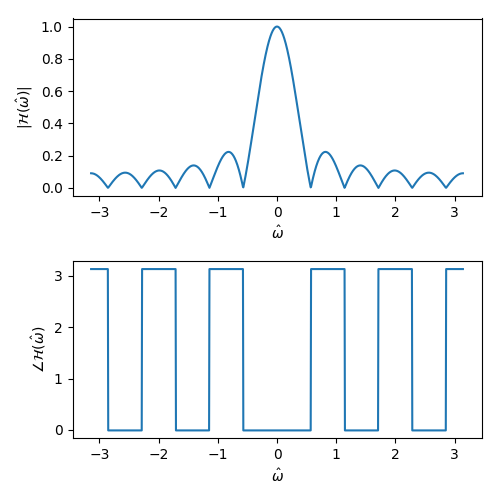
\includegraphics[width=\textwidth]{code/025_system_function/rma_magresp.png}
\end{center}
\caption{The magnitude and phase response of the running average filter.}
\label{fig:magresp}
\end{marginfigure}

\begin{figure}
\begin{center}
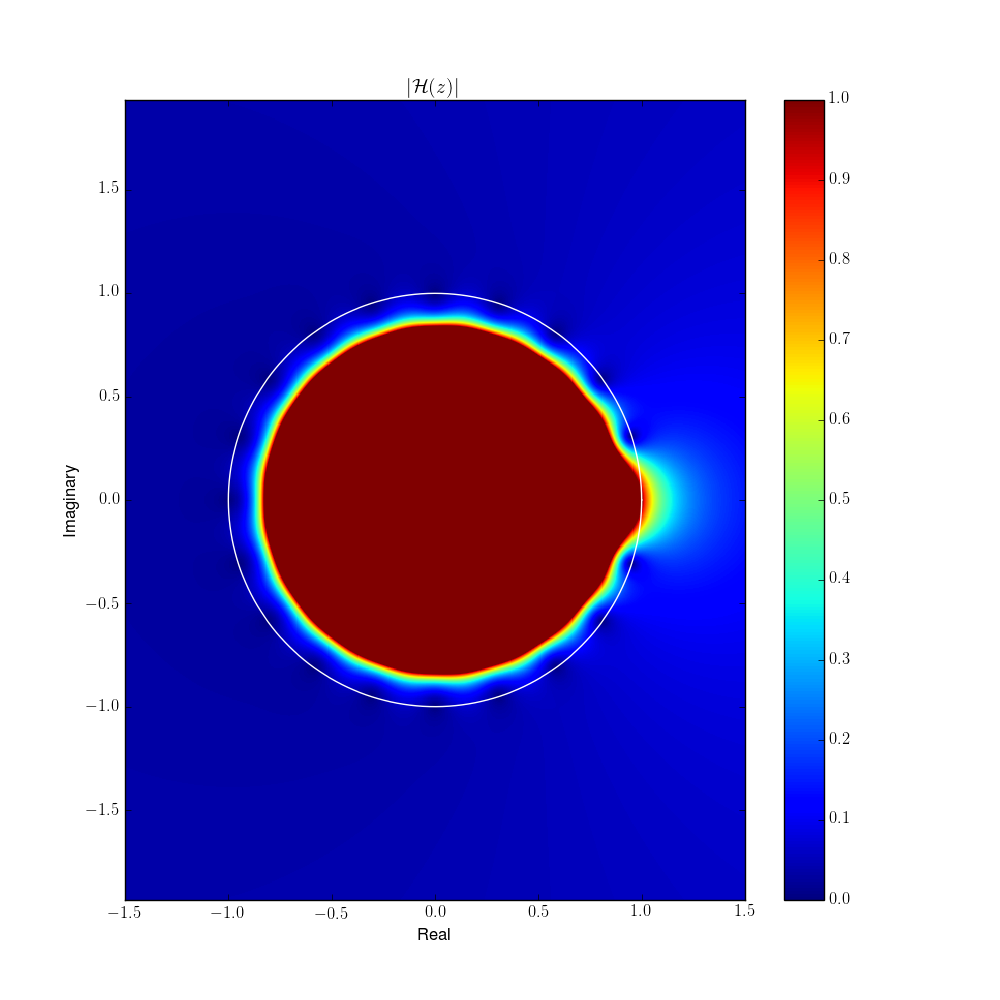
\includegraphics[width=\textwidth]{ch18/figures/zcol2.png}
\end{center}
\caption{The running average system function magnitude
  $|\mathcal{H}(z)|$ plotted on the complex plane. The $L-1$ zeros of
  the system function are evenly distributed
  $\alpha_k=e^{i\frac{2\pi}{L}k}$ with $k\in {1,2,\cdots,L-1}$. These
  are the frequencies that are perfectly cancelled out. The unit
  circle $e^{i\hat{\omega}}$ is denoted with a white line.}
\label{fig:rma_l20}
\end{figure}


\begin{figure}
\begin{center}
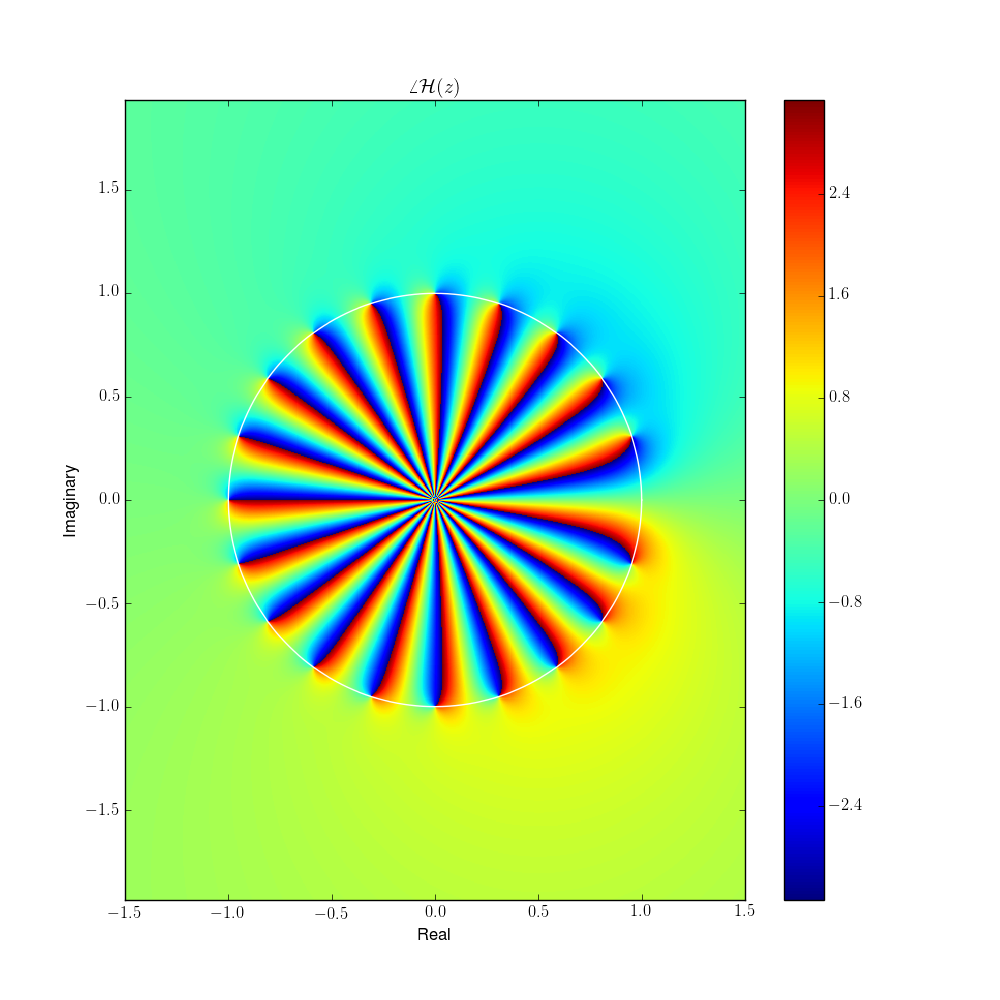
\includegraphics[width=\textwidth]{ch18/figures/zcol2p.png}
\end{center}
\caption{The phase angle of the system function corresponding to a running average filter.}
\label{fig:rma_l20_phase}
\end{figure}

If we evaluate the value of the system function on the unit circle
$z=e^{i\hat{\omega}}$, we obtain the magnitude and phase response of
the system. This is shown in Figure \ref{fig:magresp}. This is a
low-pass filter.

\fi
